\section{Introduction: An Operational Test for Concept-Aligned Supernodes}
\label{sec:intro}

\paragraph{The interpretation bottleneck.}
Attribution graphs scale faster than humans can read them. A single Gemma-2-2B-it graph for a short factual prompt routinely contains 600--5{,}000 cross-layer transcoder (CLT) features and edges between them~\cite{ameisen2025circuittracing,lindsey2025biology}. Manual interpretation by an experienced circuit tracer is reported to take approximately two hours per prompt~\cite{neuronpedia2025}. Existing autointerp pipelines~\cite{bills2023autointerp,templeton2024scaling,bricken2023monosemanticity} label individual features from corpus activations, but they do not produce \emph{circuit-level} groupings calibrated to a prompt's target logit, and they are not validated by intervention. As mechanistic interpretability moves from single circuits to large-scale catalogs~\cite{hannaameisen2026planning,marks2024dictionary}, an automated, behavior-grounded, and \emph{causally validated} grouping is needed.

\paragraph{Approach: probe prompting.}
We propose \emph{probe prompting}, a transparent rule-based pipeline that converts an attribution graph into compact subgraphs of \emph{concept-aligned supernodes}. For each candidate feature in the graph, we project a small set of concept-targeted prompts (the ``lights'') and record the per-feature Cross-Prompt Activation Signatures (CPAS) (the ``shadows''). Threshold rules then assign one of four functional roles---Semantic-Dictionary, Semantic-Concept, Relationship, Say-X---and same-role same-name features are grouped into supernodes. The pipeline is deterministic, auditable, and editable; learned classifiers were rejected because the grouping itself is the object of interpretability research and must be inspectable~\cite{rudin2019stop}.

\paragraph{An operational test, not a similarity test.}
Behavioral coherence relative to a geometric clustering baseline (cosine, layer-adjacency) is structurally biased: any grouping derived from a behavior-grounded signature outperforms a purely geometric grouping on behavior-grounded metrics, near-tautologically. \citet{heap2025sparse} sharpen this concern by showing that randomly initialized transformers can score competitively on common interpretability metrics, undermining metrics that are not anchored to causal effect. We therefore validate supernodes by \emph{intervention against structurally matched random controls}, in line with recent causal-circuit work on transcoders~\cite{hannaameisen2026planning,geiger2025causal}. We deliberately do \emph{not} claim full mechanistic identification; our supernode labels are behavioral abstractions with falsifiable causal consequences.

\paragraph{Two falsifiable claims.}
\textbf{C1 (operationally useful labels).} A supernode label is \emph{operationally useful} for entity $e$ if intervening on the supernode redirects output toward $e$ (\textbf{Specificity}, Condition~1) and a structurally matched random feature set, sampled outside concept-matching supernodes, does not (\textbf{Matched-Control}, Condition~2). \emph{Falsification:} either Specificity hit-rate fails to exceed Matched-Control hit-rate by $\geq 5$~pp on a per-pair basis, or labeled vsMax is within $1.0$ logits of Matched-Control vsMax, in any of the four strong domains (USA, Books, Products, Paintings).

\textbf{C2 (mechanistic structure surfaced by the pipeline).} The harness reveals four directional sub-claims, each with quantitative thresholds: (i) a backbone-and-specialization layer gradient (early/late Jaccard ratio $>1.4$); (ii) a less-is-more / field-interference effect (intermediate$+$answer beats all-3-fields by $\geq 10$~pp in $\geq 3/5$ domains); (iii) over-steering at the canonical $M{=}20$ default (adaptive $M$-search rescues $\geq 20\%$ of misses; high-$M$ and top-$k$ controls rescue zero); (iv) graph scaffold compatibility as a perfect ordinal predictor of domain-level hit rate across the four strong domains.

\paragraph{What we explicitly do not claim.}
Following the three-levels framing of \citet{geiger2025causal}, we claim Level~1 (operationally useful labels) and Level~2 (downstream causal effects with matched controls) but not Level~3 (full mechanistic identification of latent variables). We do not propose a new attribution method or clustering algorithm. The setting is Gemma-2-2B-it with the public CLT-HP dictionary on single-hop factual recall; cross-architecture and chain-of-thought generalization are open.

\paragraph{Contributions.}
\begin{enumerate}\itemsep0pt
  \item \textbf{Pipeline.} A transparent, rule-based pipeline that converts attribution graphs into concept-aligned supernodes from cross-prompt activation signatures (\cref{sec:method}).
  \item \textbf{Causal-validation harness.} A matched-random-control swap protocol with field-additivity decomposition and adaptive $M$-search, applicable to any feature-grouping method (\cref{sec:method}, \cref{sec:expdesign}).
  \item \textbf{Substantive findings.} Less-is-more, over-steering at $M{=}20$, and scaffold-as-predictor (\cref{sec:results}).
  \item \textbf{Open release.} A 42{,}184-run dataset, anonymous code, and an interactive demo (\cref{sec:repro}).
\end{enumerate}

\begin{figure*}[t]
  \centering
  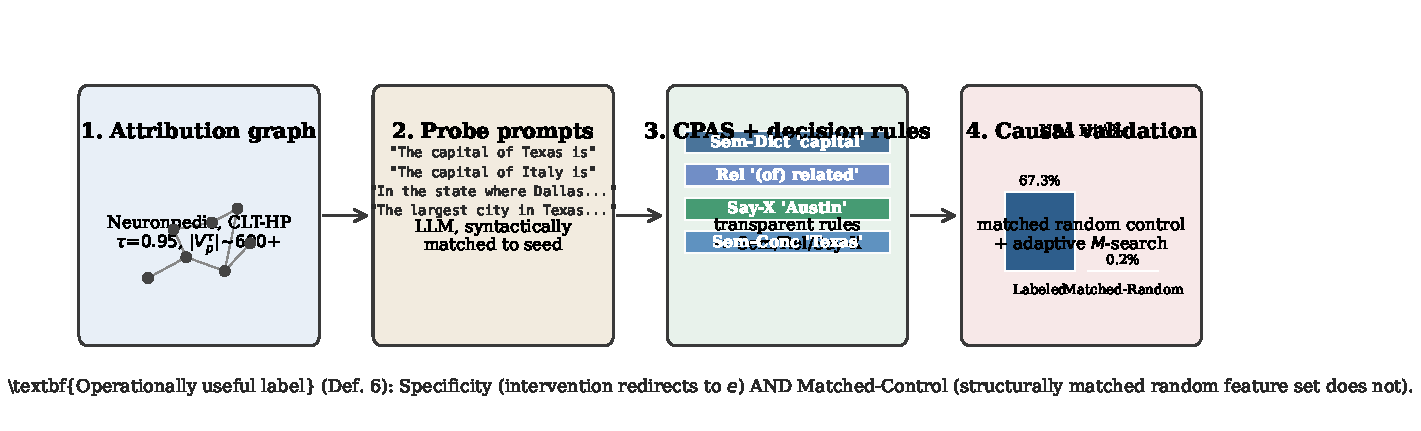
\includegraphics[width=0.95\textwidth]{figures/fig1_pipeline.pdf}
  \caption{\textbf{Pipeline overview.} Four stages: (1) attribution graph generation (Neuronpedia, CLT-HP features, $\tau{=}0.95$); (2) probe prompts (LLM-generated, syntactically matched to seed); (3) Cross-Prompt Activation Signatures and transparent decision rules $\rightarrow$ typed supernodes; (4) \textbf{causal-validation} via additive feature-swap interventions with structurally matched random controls (same feature count, same per-layer histogram, sampled outside concept-matching supernodes). The unit of analysis is the supernode, validated operationally by Conditions~1 and~2 of \cref{def:opuseful}.}
  \label{fig:pipeline}
\end{figure*}
